\subsection{Streaming de dados}
\label{sec:streaming}

	Baseando-se no objetivo do ~\textit{middleware uOS} é a adaptabilidade de serviços e a ampliação do
	protocolo de comunicação de dados ~\textit{uP} para operar em diversos tipos de aplicação, dada a grande
	heterogenidade de dispositivos ao longo do ~\textit{smart space}, Lins ~\cite{lins} propôs um novo
	protocolo de comunicação de dados baseados no ~\textit{Real-time Protocol (RTP)} e ~\textit{User
	Datagram Protocol (UDP)} para transferência de ~\textit{streaming} no ~\textit{uOS}.

	\begin{itemize}
	  \item Protocolo ~\textit{UDP}
	  	
	  	Na pilha ~\textit{TCP}/\textit{IP}, o protocolo ~\textit{UDP}, encontra-se na camada de
	  	aplicação. Tal protocolo não é orientado a conexão, ou seja, não há um estabelecimento prévio de
	  	conexão, não faz controle de fluxo, congestionamento e nem erros.
	  	
	  	Como o protocolo acaba sendo adequado a transmissão de dados em tempo real, pelo fato de não
	  	necessitar o estabelecimento prévio de conexão, algumas aplicações admitem perda de parte dos
	  	dados trafegados. Algumas utilidades do protocolo ~\textit{UDP} pode ser vista em:
	  	
	  	~\begin{enumerate}
	  	  \item ~\textit{Voice over Internet Protocol}
	  	  \item Transmissão de vídeo
	  	\end{enumerate}
	  	
	  	Pelo fato do protocolo ~\textit{UDP} não ser orientado a conexão, trouxe algumas dificuldade em
	  	sua implementação junto ao ~\textit{middleware uOS}, como por exemplo, a abstração da
	  	implementação do protocolo ~\textit{UDP} pela ~\textit{Application Programmer Interface} não
	  	suportar a abertura de múltiplas conexões.
	  	 
	  	Para contornar esse problema, foi criado um gerenciador de conexões ~\textit{UDP}, conforme
	  	visto na figura ~\ref{fig:udp}.
	  
	  	\begin{figure}[h]
			\centering 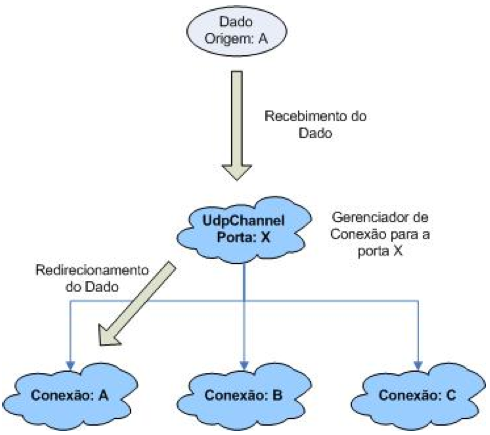
\includegraphics[scale=.55]{figuras/cap3/udpChannel.png}
			\caption{\textit{UdpChannel ~\cite{lins}}}
			\label{fig:udp} 
		\end{figure}
	
	  \item Protocolo ~\textit{RTC}
	
		De modo similar ao elucidado anteriormente, o protocolo ~\textit{RTC} enfrenta os mesmos desafios
		a serem implantados no ~\textit{middleware uOS} pelo motivo do mesmo ser implementado a partir do
		protocolo ~\textit{UDP}.
		
		Criou-se então um mecanismo de transporte de números sequências que são transmitidos com o intuito
		de facilitar a verificação se algum pacote está faltando, tendo em vista que o protocolo não é
		orientado a conexão. 
		
		Para transmissão dos pacotes de modo sincronizado, foi adicionado um outro tipo de informação
		contendo a marcação do momento, data e hora, que o pacote fora transmitido.
		
		O protocolo ~\textit{RTCP (Real-time Transport Control Protocol)} foi criado para dar maiores
		controles sobre as transmissões.
	
	\end{itemize}